\documentclass[sigconf,anonymous]{acmart}
% \documentclass[sigconf,screen|anonymous|authorVersion]{acmart}

% defining the \BibTeX command - from Oren Patashnik's original BibTeX documentation.
\def\BibTeX{{\rm B\kern-.05em{\sc i\kern-.025em b}\kern-.08emT\kern-.1667em\lower.7ex\hbox{E}\kern-.125emX}}

\usepackage{graphicx}
\renewcommand{\arraystretch}{1.3}
    
% Rights management information. 
% This information is sent to you when you complete the rights form.
% These commands have SAMPLE values in them; it is your responsibility as an author to replace
% the commands and values with those provided to you when you complete the rights form.
%
% These commands are for a PROCEEDINGS abstract or paper.
\copyrightyear{2018}
\acmYear{2018}
\setcopyright{acmlicensed}
\acmConference[Woodstock '18]{Woodstock '18: ACM Symposium on Neural Gaze Detection}{June 03--05, 2018}{Woodstock, NY}
\acmBooktitle{Woodstock '18: ACM Symposium on Neural Gaze Detection, June 03--05, 2018, Woodstock, NY}
\acmPrice{15.00}
\acmDOI{10.1145/1122445.1122456}
\acmISBN{978-1-4503-9999-9/18/06}

%
% These commands are for a JOURNAL article.
%\setcopyright{acmcopyright}
%\acmJournal{TOG}
%\acmYear{2018}\acmVolume{37}\acmNumber{4}\acmArticle{111}\acmMonth{8}
%\acmDOI{10.1145/1122445.1122456}

%
% Submission ID. 
% Use this when submitting an article to a sponsored event. You'll receive a unique submission ID from the organizers
% of the event, and this ID should be used as the parameter to this command.
%\acmSubmissionID{123-A56-BU3}
\begin{document}

\title{Role of Lipschitz constant in Gradient Learning}

%
% The "author" command and its associated commands are used to define the authors and their affiliations.
% Of note is the shared affiliation of the first two authors, and the "authornote" and "authornotemark" commands
% used to denote shared contribution to the research.
\author{Snehanshu Saha}
%\authornote{Both authors contributed equally to this research.}
\affiliation{%
  \institution{PES University}
  \city{Bengaluru}
  \state{Karnataka}
}
\email{snehanshusaha@pes.edu}
%\orcid{1234-5678-9012}

\author{Rahul Yedida}
%\authornotemark[1]
\affiliation{%
  \institution{PES University, Electronic City Campus}
  \city{Bengaluru}
  \state{Karnataka}
}
\email{y.rahul@outlook.com}

%
% The abstract is a short summary of the work to be presented in the article.
\begin{abstract}
Finding an optimal learning rate in gradient descent has typically been an empirical process. We attempt to mathematically compute an optimal value for the learning rate by exploiting functional properties of the loss function. By making only minimal assumptions about the functions, we argue that the inverse of the Lipschitz constant is this optimal value, and empirically show that this is indeed the case.
\end{abstract}

 \begin{CCSXML}
<ccs2012>
<concept>
<concept_id>10010147.10010257.10010321</concept_id>
<concept_desc>Computing methodologies~Machine learning algorithms</concept_desc>
<concept_significance>500</concept_significance>
</concept>
<concept>
<concept_id>10002950.10003714.10003716.10011138.10010043</concept_id>
<concept_desc>Mathematics of computing~Convex optimization</concept_desc>
<concept_significance>300</concept_significance>
</concept>
</ccs2012>
\end{CCSXML}

\ccsdesc[500]{Computing methodologies~Machine learning approaches}
\ccsdesc[300]{Mathematics of computing~Convex optimization}

\keywords{gradient descent, Lipschitz constant, regression, classification, learning rate, machine learning}
\maketitle

\section{Introduction}
Gradient descent is a popular optimization algorithm for finding optima for functions, and is used to find optima in loss functions in machine learning tasks. In an iterative process, it seeks to update randomly initialized weights to minimize the training error. These updates are typically small values proportional to the gradient of the loss function. The constant of proportionality is called the learning rate, and is usually manually chosen.

The gradient descent update rule is given by
\[
    \textbf{w} := \textbf{w} - \alpha \cdot \nabla_{\textbf{w}} f
\]
where $f$ is the loss function. When the learning rate, $\alpha$, is too small, then convergence takes a long time. However, when the learning rate is too large, the solution diverges. 

For a function, the Lipschitz constant is the least positive constant $L$ such that 
\[
    \left\Vert f(\textbf{w}_1) - f(\textbf{w}_2)\right\Vert \leq L \left\Vert \textbf{w}_1 - \textbf{w}_2 \right\Vert
\]
for all $\textbf{w}_1$, $\textbf{w}_2$ in the domain of $f$. From the mean-value theorem for scalar fields, for any $\textbf{w}_1, \textbf{w}_2$, there exists $\textbf{v}$ such that 

\[
    \begin{aligned}
        \left\Vert f(\textbf{w}_1) - f(\textbf{w}_2) \right\Vert &= \left\Vert \nabla_{\textbf{w}} f(\textbf{v}) \right\Vert \left\Vert \textbf{w}_1-\textbf{w}_2 \right\Vert \\
        &\leq \sup\limits_{\textbf{v}} \left\Vert \nabla_{\textbf{w}} f(\textbf{v}) \right\Vert \left\Vert \textbf{w}_1-\textbf{w}_2 \right\Vert
    \end{aligned}
\]
Thus, $\sup\limits_{\textbf{v}} \left\Vert \nabla_{\textbf{w}} f(\textbf{v}) \right\Vert$ is such an $L$. Since $L$ is the least such constant, 
\[
    L \leq \sup\limits_{\textbf{v}} \left\Vert \nabla_{\textbf{w}} f(\textbf{v}) \right\Vert
\]
In this paper, we use $\max |\nabla_{\textbf{w}} f|$ to derive the Lipschitz constants. Our approach makes the minimal assumption that the functions are Lipschitz continuous and differentiable up to first order only \footnote{Note this is a weaker condition than assuming the gradient of the function being Lipschitz continuous. We exploit merely the boundedness of the gradient.}. Because the gradient of these loss functions is used in gradient descent, these conditions are guaranteed to be satisfied.

By setting $\alpha = \frac{1}{L}$, we have $\Delta \textbf{w} \leq 1$, constraining the change in the weights. This makes it optimal to set the learning rate to the reciprocal of the Lipschitz constant. The following sections show the derivation for the Lipschitz constants for various loss functions. The derived constants are in terms of the data, which is a constant with respect to the weight vector.

% displaymath environment for unnumbered equations
% must use \Description in figures

\section{Least squares cost function} \label{lstsq}
We have,
\[
    g(\textbf{w}) = \frac{1}{2m}\sum\limits_{i=1}^m \left(\textbf{x}^{(i)} \textbf{w} - y^{(i)}\right)^2
\]
Thus,
\[
    \begin{aligned}
        g(\textbf{w}) - g(\textbf{v}) &= \frac{1}{2m}\sum\limits_{i=1}^m \left(\textbf{x}^{(i)} \textbf{w} - y^{(i)}\right)^2 - \left(\textbf{x}^{(i)} \textbf{v} - y^{(i)}\right)^2 \\
        &= \frac{1}{2m}\sum\limits_{i=1}^m \left( \textbf{x}^{(i)}(\textbf{w}+\textbf{v}) - 2y^{(i)}\right) \left( \textbf{x}^{(i)} (\textbf{w}-\textbf{v}) \right) \\
        &= \frac{1}{2m}\sum\limits_{i=1}^m \left( (\textbf{w}+\textbf{v})^T \textbf{x}^{(i)T} - 2y^{(i)}\right) \left( \textbf{x}^{(i)} (\textbf{w}-\textbf{v}) \right) \\
        &= \frac{1}{2m}\sum\limits_{i=1}^m \left( (\textbf{w} + \textbf{v})^T \textbf{x}^{(i)T}\textbf{x}^{(i)} - 2y^{(i)}\textbf{x}^{(i)} \right) (\textbf{w}-\textbf{v}) 
    \end{aligned}
\]
The penultimate step is obtained by observing that $(\textbf{w}+\textbf{v})^T \textbf{x}^{(i)T}$ is a real number, whose transpose is itself.

At this point, we take the norm on both sides, and then assume that $\textbf{w}$ and $\textbf{v}$ are bounded such that $\left\Vert \textbf{w} \right\Vert, \left\Vert \textbf{v} \right\Vert \leq K$. Taking norm on both sides,
\[
    \boxed{
        \frac{\left\Vert g(\textbf{w}) - g(\textbf{v}) \right\Vert}{\left\Vert \textbf{w} - \textbf{v} \right\Vert} \leq \frac{K}{m}\left\Vert \textbf{X}^T\textbf{X} \right\Vert - \frac{1}{m} \left\Vert\textbf{y}^T \textbf{X} \right\Vert
    }
\]
We are forced to use separate norms because the matrix subtraction $2K \textbf{X}^T\textbf{X} - 2\textbf{y}^T \textbf{X}$ cannot be performed. 
The RHS here is the Lipschitz constant. Note that the Lipschitz constant changes if the cost function is considered with a factor other than $\frac{1}{2m}$.

\subsection{An alternate derivation}
The least-squares system can also be formulated as 
\[
    \begin{aligned} L(\textbf{w}) &= \left\Vert \textbf{X}\textbf{w} - \textbf{y} \right\Vert \\ &= (\textbf{X}\textbf{w} - \textbf{y})^T (\textbf{X}\textbf{w} - \textbf{y}) \end{aligned}
\]
Then, we have
\[
    \begin{aligned}
			L(\textbf{b}) - L(\textbf{a}) =& \left( X\textbf{b} - Y \right)^T (X\textbf{b} - Y) - (X\textbf{a} - Y)^T (X\textbf{a} - Y) \\
			=& (\textbf{b}^T X^T - Y^T)(X\textbf{b} - Y) - (\textbf{a}^T X^T - Y^T)(X\textbf{a} - Y) \\
			=& \textbf{b}^T X^T X \textbf{b} - \textbf{b}^T X^T Y - Y^T X\textbf{b} + Y^T Y - \textbf{a}^T X^T X\textbf{a} + \\ &\textbf{a}^T X^T Y + Y^T X\textbf{a} - Y^T Y \\
			=& \textbf{b}^T X^T X \textbf{b} - \textbf{b}^T X^T Y - Y^T X\textbf{b} - \textbf{a}^T X^T X\textbf{a} + \\
			& \textbf{a}^T X^T Y + Y^T X\textbf{a} \\
			=& \textbf{b}^T X^T X \textbf{b} - 2Y^T X\textbf{b} - \textbf{a}^T X^T X\textbf{a} + 2Y^T X\textbf{a} \\
			=& \textbf{b}^T X^T X \textbf{b} - \textbf{a}^T X^T X\textbf{a} - 2Y^T X(\textbf{b} - \textbf{a}) \\
			=& (\textbf{b} - \textbf{a} + \textbf{a})^T X^T X \textbf{b} - \textbf{a}^T X^T X\textbf{a} - 2Y^T X(\textbf{b} - \textbf{a}) \\
			=& (\textbf{b} - \textbf{a})^T X^T X \textbf{b} + \textbf{a}^T X^T X \textbf{b} - \textbf{a}^T X^T X\textbf{a} \\
			& - 2Y^T X(\textbf{b} - \textbf{a}) \\
			=& (\textbf{b} - \textbf{a})^T X^T X \textbf{b} + \textbf{a}^T X^T X (\textbf{b} - \textbf{a}) - 2Y^T X(\textbf{b} - \textbf{a}) \\
			=& (\textbf{b} - \textbf{a})^T X^T X (\textbf{b} - \textbf{a} + \textbf{a}) + \textbf{a}^T X^T X (\textbf{b} - \textbf{a}) \\
			& - 2Y^T X(\textbf{b} - \textbf{a}) \\
			=& (\textbf{b} - \textbf{a})^T X^T X\textbf{a} + \textbf{a}^T X^T X(\textbf{b} - \textbf{a}) + \\
			& (\textbf{b} - \textbf{a})^T X^T X(\textbf{b} - \textbf{a}) - 2Y^T X(\textbf{b} - \textbf{a}) \\
			=& \textbf{a}^T X^T X (\textbf{b} - \textbf{a}) + \textbf{a}^T X^T X(\textbf{b} - \textbf{a}) + \\
			& (\textbf{b} - \textbf{a})^T X^T X(\textbf{b} - \textbf{a}) - 2Y^T X(\textbf{b} - \textbf{a}) \\
			=& 2\textbf{a}^T X^T X(\textbf{b} - \textbf{a}) + (\textbf{b} - \textbf{a})^T X^T X(\textbf{b} - \\
			& \textbf{a}) - 2Y^T X(\textbf{b} - \textbf{a})
		\end{aligned}
\]
The triangle inequality now gives us,
\[
    \frac{\left\Vert L(\textbf{b}) - L(\textbf{a}) \right\Vert}{\left\Vert \textbf{b} - \textbf{a} \right\Vert} \leq 2 \left\Vert \textbf{a} \right\Vert \left\Vert X^T X \right\Vert - 2\left\Vert Y^T X \right\Vert + \left\Vert \textbf{b} - \textbf{a} \right\Vert \left\Vert X^T X \right\Vert
\]
Assuming $\left\Vert \textbf{a} \right\Vert, \left\Vert \textbf{b} \right\Vert \leq K$,
\[
    \frac{\left\Vert L(\textbf{b}) - L(\textbf{a}) \right\Vert}{\left\Vert \textbf{b} - \textbf{a} \right\Vert} \leq 2K \left\Vert X^T X \right\Vert - 2 \left\Vert Y^T X \right\Vert
\]
and so we can set the Lipschitz constant to
\[
    \boxed{
        L = 2K \left\Vert X^T X \right\Vert - 2 \left\Vert Y^T X \right\Vert
    }
\]
\section{Binary cross-entropy function}
We have,
\[
    g(\textbf{w}) = \frac{1}{m}\sum\limits_{i=1}^m -y^{(i)}\log h(x^{(i)}) - (1-y^{(i)})\log \left( 1 - h(x^{(i)}) \right) 
\]
where $h(x^{(i)}) = \frac{1}{1+e^{-\textbf{w}^T \textbf{x}^{(i)}}}$.

We have,
\[
    \begin{aligned}
        \frac{\partial h(\textbf{x}^{(i)})}{\partial \textbf{w}_j} &= -\frac{e^{-\textbf{w}^T \textbf{x}^{(i)}} \left( -x^{(i)}_j \right)}{1+e^{-\textbf{w}^T \textbf{x}^{(i)}}} \\
        &= \frac{1}{1+e^{-\textbf{w}^T \textbf{x}^{(i)}}}\cdot \left( 1 - \frac{1}{1+e^{-\textbf{w}^T \textbf{x}^{(i)}}} \right) \cdot x^{(i)}_j \\
        &= h(\textbf{x}^{(i)}) \left( 1 - h(\textbf{x}^{(i)}) \right)x^{(i)}_j
    \end{aligned}
\]

The gradient is then,
\[
    \begin{aligned} \frac{\partial}{\partial \textbf{w}_j} g(\textbf{w}) &= \frac{\partial}{\partial \textbf{w}_j} \left( \frac{-1}{m} \sum_{i = 1}^m y^{(i)} \log \left( h(\textbf{x}^{(i)}) \right) + (1 - y^{(i)}) \log \left( 1 - h(\textbf{x}^{(i)}) \right) \right) \\ 
    &= \frac{-1}{m} \sum_{i = 1}^m \left( \frac{y^{(i)}}{h(\textbf{x}^{(i)})}h^{\prime}(\textbf{x}^{(i)}) + \frac{1 - y^{(i)}}{1 - h(\textbf{x}^{(i)})}(-h^{\prime}(\textbf{x}^{(i)})) \right) \\ 
    &= \frac{-1}{m} \sum_{i = 1}^m \left( y^{(i)}(1 - h(\textbf{x}^{(i)}))(\textbf{x}^{(i)}_j) - (1 - y^{(i)})h(\textbf{x}^{(i)})(x^{(i)}_j) \right) \\ 
    &= \frac{-1}{m} \sum_{i = 1}^m \left( y^{(i)}(1 - h(\textbf{x}^{(i)})) - (1 - y^{(i)})h(\textbf{x}^{(i)}) \right)x^{(i)}_j \\ 
    &= \frac{1}{m} \sum_{i = 1}^m \left( y^{(i)} - y^{(i)}h(\textbf{x}^{(i)}) - h(\textbf{x}^{(i)}) + y^{(i)}h(\textbf{x}^{(i)}) \right)x^{(i)}_j \\ 
    &= \frac{1}{m} \sum_{i = 1}^m \left( h(\textbf{x}^{(i)}) - y^{(i)} \right)x^{(i)}_j \end{aligned}
\]
It is trivial to show that the maximum of this occurs when $h(\textbf{x}^{(i)})=\frac{1}{2}$: for any $k$,
\[
    \begin{aligned}
        \frac{\partial}{\partial \textbf{w}_k} \left( h(\textbf{x}^{(i)}) - y^{(i)} \right)x^{(i)}_j &= \frac{\partial}{\partial \textbf{w}_k} h(\textbf{x}^{(i)})x^{(i)}_j \\
        &= h(\textbf{x}^{(i)})\left(1-h(\textbf{x}^{(i)}) \right)x^{(i)}_k x^{(i)}_j
    \end{aligned}
\]
Within the domain $(-\infty, \infty)$, the first two terms cannot be 0; the last term is a constant, and thus $x^{(i)}_k = 0$, and thus $h(\textbf{x}^{(i)}) = \frac{1}{2}$. Now whether $y^{(i)}$  is 0 or 1, $\lvert h(\textbf{x}^{(i)}) - y^{(i)} \rvert = \frac{1}{2}$.

Thus, the Lipschitz constant is
\[
    \boxed{
        L = \frac{1}{2m} \left\Vert \textbf{X} \right\Vert
    }
\]

\section{Cross-entropy loss function} 
The cross-entropy loss (or softmax loss) is defined as \footnotetext{This version of the softmax loss assumes the labels are distributed according to a Multinomial distribution. Later, we will show that even when the output is assumed to be one-hot encoded, the Lipschitz constant remains the same.}
\[
    g(\textbf{w}) = -\frac{1}{m} \sum\limits_{i=1}^m \sum\limits_{j=1}^k [y^{(i)}=j] \log \left( \frac{e^{\boldsymbol\Theta_j^T \textbf{x}^{(i)}}}{\sum_{l=1}^k e^{\boldsymbol\Theta_l^T \textbf{x}^{(i)}}} \right)
\]
Here, we are using the Iverson notation: the expression $[y^{(i)}=j]$ is 1 if the condition is true, and 0 otherwise. To find the Lipschitz constant, we require the derivative of the softmax function, which is the fraction in the log term.
\[
    \begin{aligned} \frac{\partial s_j}{\partial \boldsymbol\Theta_p} &= \frac{\partial}{\partial \boldsymbol\Theta^T_p \textbf{x}^{(i)}} \left( \frac{e^{\boldsymbol\Theta^T_j \textbf{x}^{(i)}}}{\sum_{l=1}^k e^{\boldsymbol\Theta^T_l \textbf{x}^{(i)}}} \right) \cdot \frac{\partial}{\partial \boldsymbol\Theta_p} \left( \boldsymbol\Theta^T_p \textbf{x}^{(i)} \right)  \\ &= \frac{[p=j] e^{\boldsymbol\Theta^T_j \textbf{x}^{(i)}}\sum_{l=1}^k e^{\boldsymbol\Theta^T_l \textbf{x}^{(i)}} - e^{\boldsymbol\Theta^T_j \textbf{x}^{(i)}} \cdot e^{\boldsymbol\Theta^T_p \textbf{x}^{(i)}} }{\left( \sum_{l=1}^k e^{\boldsymbol\Theta^T_l \textbf{x}^{(i)}} \right)^2} \cdot \textbf{x}^{(i)} \\ &= \left( \frac{[p=j] e^{\boldsymbol\Theta^T_j \textbf{x}^{(i)}}}{\sum_{l=1}^k e^{\boldsymbol\Theta^T_l \textbf{x}^{(i)}}} - \frac{e^{\boldsymbol\Theta^T_j \textbf{x}^{(i)}}}{\sum_{l=1}^k e^{\boldsymbol\Theta^T_l \textbf{x}^{(i)}}} \cdot \frac{e^{\boldsymbol\Theta^T_p \textbf{x}^{(i)}}}{\sum_{l=1}^k e^{\boldsymbol\Theta^T_l \textbf{x}^{(i)}}} \right) \cdot \textbf{x}^{(i)} \\ &= \left([p=j] s_j - s_j s_p \right) \cdot \textbf{x}^{(i)} \\ &= s_j([p=j]-s_p)\textbf{x}^{(i)} \end{aligned}
\]
We use the notation $s_j$ to denote the softmax function. The first step uses the chain rule for derivatives. The second step is obtained by applying the quotient rule and noting that the partial derivative is taken with respect to $\boldsymbol\Theta_p^T \textbf{x}^{(i)}$. We then simplify, split the fraction into two, and cancel out terms. In a more concise fashion, we write the above result as:
\begin{equation}
    \frac{\partial s_j}{\partial \boldsymbol\Theta_p} = s_j([p=j]-s_p)\textbf{x}^{(i)} \label{softmax:1}
\end{equation}
We can now use \eqref{softmax:1} to find the gradient of $g$.
\[
    \begin{aligned}
        \nabla_{\boldsymbol\Theta_p} g =& -\frac{1}{m} \sum\limits_{i=1}^m \sum\limits_{j=1}^k \nabla_{\boldsymbol\Theta_p} [y^{(i)}=j]\log s_j \\
        =& -\frac{1}{m} \sum\limits_{i=1}^m \sum\limits_{j=1}^k \frac{[y^{(i)}=j]}{s_j} \nabla_{\boldsymbol\Theta_p} s_j \\
        =& -\frac{1}{m} \sum\limits_{i=1}^m \sum\limits_{j=p} [y^{(i)}=j] (1-s_p)\textbf{x}^{(i)} - \\
        & \frac{1}{m} \sum\limits_{i=1}^m \sum\limits_{j \neq p} [y^{(i)}=j](-s_p)\textbf{x}^{(i)} \\
        =& -\frac{1}{m} \sum\limits_{i=1}^m \sum\limits_{j=p} [y^{(i)}=j]\textbf{x}^{(i)} + \frac{1}{m} \sum\limits_{i=1}^m \sum\limits_{j=p} [y^{(i)}=j]s_p \textbf{x}^{(i)} + \\
        & \frac{1}{m} \sum\limits_{i=1}^m \sum\limits_{j \neq p} [y^{(i)}=j]s_p \textbf{x}^{(i)} \\
        =& -\frac{1}{m} \sum\limits_{i=1}^m [y^{(i)}=p]\textbf{x}^{(i)} + \frac{1}{m} \sum\limits_{i=1}^m [y^{(i)}=p]s_p \textbf{x}^{(i)} + \\
        & \frac{1}{m} \sum\limits_{i=1}^m [y^{(i)} \neq p] s_p \textbf{x}^{(i)} \\
        =& -\frac{1}{m} \sum\limits_{i=1}^m [y^{(i)}=p]\textbf{x}^{(i)} + \\
        & \frac{1}{m} \sum\limits_{i=1}^m s_p \textbf{x}^{(i)} \left( [y^{(i)}=p] + [y^{(i)} \neq p] \right) \\
        =& -\frac{1}{m} \sum\limits_{i=1}^m [y^{(i)}=p]\textbf{x}^{(i)} + \frac{1}{m} \sum\limits_{i=1}^m s_p \textbf{x}^{(i)}
    \end{aligned}
\]
Thus,
\begin{equation}
    \nabla_{\boldsymbol\Theta_p} g = \frac{1}{m} \sum\limits_{i=1}^m \textbf{x}^{(i)} \left(s_p - [y^{(i)}=p] \right) \label{softmax:2}
\end{equation}

In the limiting case, all the softmax values are equal, and $y^{(i)} = p$; for $k$ classes, $s_p = \frac{1}{k}$, yielding $|s_p-1| = \frac{k-1}{k}$ so we get the inequality

\begin{equation}
    |[y^{(i)} = p](s_p-1)| \leq \frac{k-1}{k} \label{softmax:3}
\end{equation}
Using \eqref{softmax:3} in \eqref{softmax:2}, we get
\[
    |\nabla_{\boldsymbol\Theta_p} g| \leq \frac{k-1}{km} \sum\limits_{i=1}^m \textbf{x}^{(i)}
\]
and thus we obtain the Lipschitz constant for the softmax loss function:

\[
    \boxed{
        L = \frac{k-1}{km}\left\Vert \textbf{X} \right\Vert
    }
\]

\section{A note on regularization} \label{regularization}
It should be noted that this framework is extensible to the case where the loss function includes a regularization term. 

In particular, if an $L_2$ regularization term, $\frac{\lambda}{2}\left\Vert \textbf{w} \right\Vert_2^2$ is added, it is trivial to show that the Lipschitz constant increases by $\lambda K$, where $K$ is the upper bound for $\left\Vert \textbf{w} \right\Vert$. More generally, if a Tikhonov regularization term, $\left\Vert \boldsymbol\Gamma \textbf{w} \right\Vert_2^2$ term is added, then the increase in the Lipschitz constant can be computed in the same way as shown in the alternate derivation for the least-squares loss above. For the sake of continuity, we show a succinct version of the derivation below:

\[
    \begin{aligned}
        L(\textbf{w}_1) - L(\textbf{w}_2) &= (\boldsymbol\Gamma \textbf{w}_1)^T (\boldsymbol\Gamma \textbf{w}_1) - (\boldsymbol\Gamma \textbf{w}_2)^T (\boldsymbol\Gamma \textbf{w}_2) \\
        &= \textbf{w}_1^T \boldsymbol\Gamma^2 \textbf{w}_1 - \textbf{w}_2^T \boldsymbol\Gamma^2 \textbf{w}_2 \\
        &= 2\textbf{w}_2^T \boldsymbol\Gamma^2 (\textbf{w}_1 - \textbf{w}_2) + (\textbf{w}_1-\textbf{w}_2)^T \Gamma^2 (\textbf{w}_1-\textbf{w}_2) \\
        \frac{\left\Vert L(\textbf{w}_1) - L(\textbf{w}_2) \right\Vert}{\left\Vert \textbf{w}_1-\textbf{w}_2 \right\Vert} & \leq 2 \left\Vert \textbf{w}_2 \right\Vert \left\Vert \boldsymbol\Gamma^2 \right\Vert + \left\Vert \textbf{w}_1-\textbf{w}_2 \right\Vert \left\Vert \boldsymbol\Gamma^2 \right\Vert 
    \end{aligned}
\]

Now by the assumption that $\textbf{w}_1, \textbf{w}_2$ are bounded by $K$, 

\[
    \boxed{
        L = 2K \left\Vert \boldsymbol\Gamma^2 \right\Vert
    }
\]

This additional term may be added to the Lipschitz constants derived above when gradient descent is performed on a loss function including a Tikhonov regularization term. Clearly, for an $L_2$-regularizer, since $\boldsymbol\Gamma = \frac{\lambda}{2}\textbf{I}$, $L = \lambda K$.

\section{Experiments}
This section discusses experiments demonstrating the faster convergence with our approach. 

In each experiment, we randomly initialize weights, and use the same initial weight vector for gradient descent with both the learning rates. In all experiments, we scale each feature to sum to 1 before running gradient descent. This scaled data is used to compute the Lipschitz constants, and consequently, the learning rates. Normalizing the data is particularly important because the Lipschitz constant may get arbitrarily large, thus making the learning rate too small.

Note that the results below are obtained from simple, computationally inexpensive models: the regression experiments use a multiple linear regression model, the binary classification experiments use an ordinary logistic regression model, and the multi-class classification experiments use a softmax regression model with one-hot encoded target labels. For MNIST, however, we found it quicker to train a neural network with only an input and output layer (no hidden layers were used), a stochastic gradient descent optimizer, and softmax activations.

\begin{figure}
    \centering
    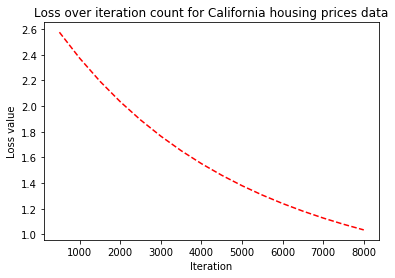
\includegraphics[scale=0.5]{cali.png}
    \caption{Loss function over iterations for California housing prices dataset}
    \label{fig:leastsq:1}
\end{figure}

\subsection{Regression experiments} \label{regexpts}
Rather than wait for absolute convergence, which may take many iterations, we instead choose to set a threshold for the value of the loss function. When the value of the cost function goes below this threshold, we stop the gradient descent procedure. A reasonable threshold value is chosen for each dataset separately.

For the least-squares cost function, an estimate of $K$ is required. A good estimate of $K$ would be obtained by running gradient descent with some fixed learning rate and then taking the norm of the final weight vectors. However, because this requires actually running the algorithm for which we want to find a parameter first, we need to estimate this value instead. In our experiments, we obtain a close approximation to the value obtained above through the formula below. For the experiments in this subsection, we use this formula to compute $K$.

\[
    \begin{aligned}
        a &= \frac{1}{m}\sum\limits_{j=1}^n \sum\limits_{i=1}^m x^{(i)}_j \\
        b &= \frac{1}{n}\sum\limits_{j=1}^n \max\limits_i x^{(i)}_j \\
        K &= \frac{a+b}{2}
    \end{aligned}
\]
In the above formulas, the notation $x^{(i)}_j$ refers to the $j$th column of the $i$th training example. Note that $a$ is the sum of the means of each column, and $b$ is the mean of the maximum of each column.

\begin{table*}
    \caption{Regression experiments on various datasets with $\alpha=0.1$ and $\alpha=\frac{1}{L}$}
    \centering
    \begin{tabular}{ccccc}
        \toprule
        Dataset & Loss threshold & Inverse Lipschitz constant & \#it with $\alpha=0.1$ & \#it with $\alpha=\frac{1}{L}$ \\
        \midrule
        Boston housing prices & 200 & 9.316 & 46,041 & 555 \\
        California housing prices & 2.8051 & 5163.5 & 24,582 & 2 \\
        Energy efficiency \cite{tsanas2012accurate} & 100 & 12.78 & 489,592 & 3,833 \\
        Online news popularity \cite{fernandes2015proactive} & 73,355,000 & 1.462 & 10,985 & 753 \\
        \bottomrule
     \end{tabular}
    \label{tab:leastsq:1}
\end{table*}

Table \ref{tab:leastsq:1} shows the results of our experiments on some datasets. Clearly, our choice of $\alpha$ outperforms a random guess in all the datasets. Our proposed method yields a learning rate that adapts to each dataset to converge significantly faster than with a guess. In some datasets, our choice of learning rate gives over a 100x improvement in training time.

While the high learning rates may raise concerns of oscillations rather than convergence, we have checked for this in our experiments. To do this, we continued running gradient descent, monitoring the value of the loss function every 500 iterations. Figure \ref{fig:leastsq:1} shows this plot, demonstrating that the high learning rates indeed lead to convergence.

\subsection{Binary classification experiments}
For classification, our experiments were conducted by running gradient descent for 1000 iterations, and then comparing accuracy scores over the two learning rates. Table \ref{tab:classif:1} summarizes the results of these experiments. Note that even with high learning rates, the algorithm outperforms a small choice of learning rate. We also ran experiments in the same manner as we did for regression: we set a reasonable error threshold and compared the number of iterations required across both learning rates. Table \ref{tab:classif:3} summarizes the results of these experiments.

For the iris dataset, we removed one class to make the problem a binary classification one. For the covertype data, we considered only the first two out of seven classes. This resulted in 495,141 rows. We also considered only ten features to speed up computation time.

\begin{table*}
    \caption{Binary classification experiments on various datasets with $\alpha=0.1$ and $\alpha=\frac{1}{L}$}
    \centering
    \begin{tabular}{cccc}
        \toprule
        Dataset & Inverse Lipschitz constant & Accuracy with $\alpha=0.1$ & Accuracy with $\alpha=\frac{1}{L}$ \\
        \midrule
        Iris & 830.22 & 50\% & 100\% \\
        Covertype & 189.35M & 43.05\% & 57.21\% \\
        Breast cancer & 4280.22 & 43.23\% & 90.5\% \\
        \bottomrule
    \end{tabular}
    \label{tab:classif:1}
\end{table*}

\subsection{Multi-class classification experiments}
For multi-class classification, the experiments were conducted in the same manner as for binary classification. However, we did not scale the data in this case. Further, the target variable was one-hot encoded before running gradient descent. Finally, we ran gradient descent for 200 iterations, rather than 1000. Table \ref{tab:classif:2} summarizes the results of these experiments.

\begin{table*}
    \caption{Softmax classification experiments on various datasets with $\alpha=0.1$ and $\alpha=\frac{1}{L}$}
    \centering
    \begin{tabular}{cccc}
        \toprule
        Dataset & Inverse Lipschitz constant & Accuracy with $\alpha=0.1$ & Accuracy with $\alpha=\frac{1}{L}$ \\
        \midrule
        Iris & 1.936 & 93.33\% & 97.78\% \\
        Digits & 0.635 & 91.3\% & 94.63\% \\
        \bottomrule
    \end{tabular}
    \label{tab:classif:2}
\end{table*}

\begin{table*}
    \caption{Classification experiments on various datasets with an error threshold}
    \centering
    \begin{tabular}{cccccc}
        \toprule
        Dataset & Loss function & Loss threshold & Inverse Lipschitz constant & \#it with $\alpha=0.1$ & \#it with $\alpha=\frac{1}{L}$ \\
        \midrule
        Breast cancer & Binary cross-entropy & 0.69 & 4280.23 & 37,008 & 2 \\
        Covertype\footnotemark & Binary cross-entropy & 0.69314 & 17.48M & 216,412 & 2 \\
        Iris & Softmax & 0.2 & 1.902 & 413 & 49 \\
        Digits & Softmax & 0.2 & 0.634 & 337 & 2 \\
        \bottomrule
    \end{tabular}
    \label{tab:classif:3}
\end{table*}

\footnotetext{The learning rate obtained here is different because we restricted the data to the first 100K rows only.}

\subsubsection{MNIST}
For MNIST, we handled the data differently. Because running gradient descent caused overflows even for learning rates of $10^{-4}$, we standardized the data first. Further, we compared the training and validation accuracy scores across both the learning rates.

Figure \ref{fig:classif:1} shows a comparative plot of the training and validation accuracy scores for both learning rates. In both the plots, the red line is for $\alpha = 0.1$, while the green line is for $\alpha = \frac{1}{L}$. Although our choice of learning rate starts off worse, it quickly (< 100 iterations) outperforms a learning rate of 0.1. 

Fig \ref{fig:classif:2} shows the training and validation accuracy scores for the same learning rates. In this figure, the y-axis is shared for easy comparison. With the higher learning rate of 10.24, our model shows a greater overfitting tendency. However, neither of these models used any regularization, and this tendency will reduce on including a regularization term in the loss function.

Finally, Table \ref{tab:classif:4} shows the number of iterations required to reach certain accuracy thresholds with each learning rate.

\begin{table}
    \caption{Iterations required to reach accuracy thresholds in MNIST experiments}
    \centering
    \begin{tabular}{ccc}
        \toprule
        Accuracy threshold & \# it with $\alpha=0.1$ & \# it with $\alpha=\frac{1}{L}$ \\
        \midrule
        92.5\% & 11 & 33 \\
        92.6\% & 22 & 58 \\
        92.7\% & 22 & 63 \\
        92.8\% & -- & 173 \\
        \bottomrule
    \end{tabular}
    \label{tab:classif:4}
\end{table}

\begin{figure}
    \centering
    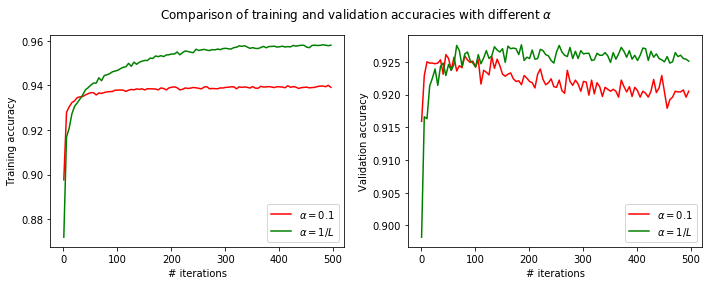
\includegraphics[scale=0.33]{mnist_acc.png}
    \caption{Comparison of training and validation accuracy scores for different $\alpha$}
    \label{fig:classif:1}
\end{figure}

\begin{figure}
    \centering
    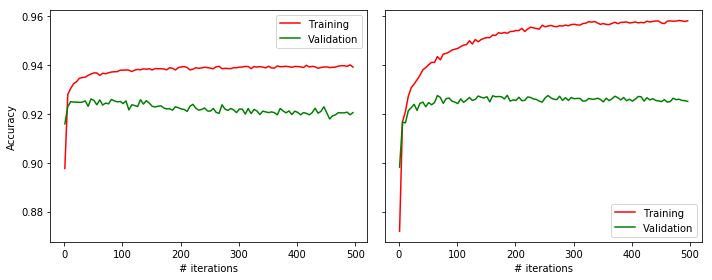
\includegraphics[scale=0.33]{mnist_train_val.png}
    \caption{Comparison of training and validation accuracy scores for same $\alpha$}
    \label{fig:classif:2}
\end{figure}

\begin{itemize}
    \item check if this softmax derivation applies to one-hot encoding as well
    \item report class-wise accuracy and other performance metrics
\end{itemize}

\section{Conclusion and Future Work}
Our major contribution in this paper is the presentation of a novel framework for automatically choosing a suitable learning rate in gradient descent. We then derived the formulas for some common loss functions. This is equally applicable, of course, to both batch and stochastic gradient descent. Our experiments confirmed that our choice of learning rate indeed leads to significantly faster convergence, as predicted by the theory.

Future work in this direction is two-fold. First, we need to investigate the utility of a similar approach in the Broyden–Fletcher–Goldfarb–Shanno (BFGS)\cite{broyden1970convergence}\cite{fletcher1970new}\cite{goldfarb1970family}\cite{shanno1970conditioning} optimization algorithm, which uses an approximation of the Hessian matrix. In BFGS, a suitable step size is chosen via line search; however, this is computationally expensive. Identifying a more direct approach to this would be considerably beneficial.

Second, this work discussed, in section \ref{regexpts}, a set of equations for computing an approximation to $K$. In our experiments, the approximation was quite close to the value of $\left\Vert \textbf{w} \right\Vert$ obtained after running gradient descent. In applications where time and/or resources are limited, an approximation to the weight vector may be sufficient. Mathematically, the equation $\left\Vert \textbf{w} \right\Vert = K$ represents an n-ball. Therefore, it may suffice to only search the surface of this n-ball, rather than the entire n-dimensional space via gradient descent. The optimization objective, therefore, is
\[
    \begin{aligned}
        \min\limits_{\textbf{w}} & J(\textbf{w}) \\
        \text{s.t. } & \left\Vert \textbf{w} \right\Vert = K 
    \end{aligned}
\]
where $J$ is some loss function. Although our constraint is non-convex, this is similar to the optimization problem in Support Vector Machines (SVMs), and future work could investigate possible approaches to solving this optimization problem.

Alternatively, the surface of the n-ball could be used to initialize weights--rather than initialize the weight vector randomly in the entire n-space, one could initialize the weights at a random point on the n-ball.

\bibliographystyle{ACM-Reference-Format}
\bibliography{citations}

\end{document}
